\section{Introduction}
\subsection{Background and Motivation}
Most startups fail for reasons that are visible early: a weak problem, a small or crowded market, unrealistic costs, or regulatory exposure [1]. Experienced venture analysts check these systematically, but students, first-time founders and small accelerator cohorts rarely have that capacity. Transformer-based large language models (LLMs) [2] make fast analysis possible, yet a single-prompt assistant has two weaknesses in this setting. First, it may state market sizes and competitor facts that are not grounded in any source, a known form of hallucination [3]. Second, it rarely signals the boundaries of its own competence; although LLMs can partly estimate when they are right [4], a chat answer gives the same confident tone to a hackathon idea and to a funded company.

\subsection{Problem Statement}
Given a startup idea, a founder stage and a set of target countries, the system must produce an analysis that is (i) grounded in retrieved evidence, (ii) decomposed so that each aspect (market, feasibility, risk, finance, pitch, execution) is handled by a specialist, and (iii) explicit about uncertainty and fit to the founder's stage.

\subsection{Objectives and Contributions}
VentureOS aims to ground early analysis in live web evidence following the retrieval-augmented generation (RAG) paradigm [5], to run independent analyses in parallel, to express limits through numeric scores, bands and structured fields, and to adapt advice and cost estimates to founder stage and geography. The main contributions are: (1) a dependency-ordered DAG of twelve agents with shared, retrieval-grounded context; (2) a ten-factor weighted risk model with explicit decision bands; (3) geography-aware market and burn-rate estimation; (4) stage-aware guardrails; and (5) a streaming full-stack implementation in which each agent result reaches the user as soon as it completes. Table~I contrasts this design with a single-prompt assistant.

\begin{table}[!t]
\caption{Single-Prompt Assistant vs. VentureOS}
\centering\footnotesize
\begin{tabularx}{\columnwidth}{@{}l>{\raggedright\arraybackslash}X@{}}\toprule
\textbf{Aspect} & \textbf{Single prompt $\rightarrow$ VentureOS}\\\midrule
Evidence & Model memory $\rightarrow$ live web retrieval\\
Structure & One free-text answer $\rightarrow$ 12 specialist agents\\
Uncertainty & Implicit $\rightarrow$ scores, bands, structured fields\\
Geography & Global averages $\rightarrow$ per-country sizing and cost\\
Founder stage & Same advice $\rightarrow$ stage-specific guidance\\\bottomrule
\end{tabularx}
\end{table}

The rest of the paper is organised as follows: Section~II reviews related work, Section~III presents the methodology, Section~IV discusses results and limitations, and Section~V concludes.

\section{Related Work}
RAG combines a parametric generator with non-parametric retrieval so that answers can draw on external evidence [5]; surveys catalogue its design choices [6], and dense retrievers underpin many systems [7]. Retrieval augmentation reduces hallucination in dialogue [8], and ReAct-style prompting interleaves reasoning with tool calls such as search [9]. Multi-agent frameworks assign roles to cooperating LLM agents: AutoGen [10], MetaGPT [11] and generative agents [12]. VentureOS applies role specialisation to venture analysis, uses a fixed DAG instead of free-form conversation, and adds a quantitative risk model. It uses Llama~3 [13] and Gemini [14].

\section{Methodology}
\subsection{System Architecture and Agent DAG}
The Next.js~16 client forwards \texttt{/api/*} calls through a reverse proxy to a FastAPI backend [15] (Fig.~1). The backend calls Groq-hosted LLaMA~3.3 70B as primary model, Gemini~2.0 Flash as fallback and for synthesis, and Serper for web search; Redis keeps one-hour sessions and MongoDB Atlas stores analyses and risk history. The core pipeline runs in four dependency-ordered batches (Fig.~2): the Research Agent retrieves market, competitor and regulatory evidence that is injected into every downstream prompt; Market Analysis and Feasibility run in parallel; the Risk Agent, which also searches the web, consumes their outputs; and the Synthesizer fuses everything into an overall venture score.

\begin{figure}[!t]
\centering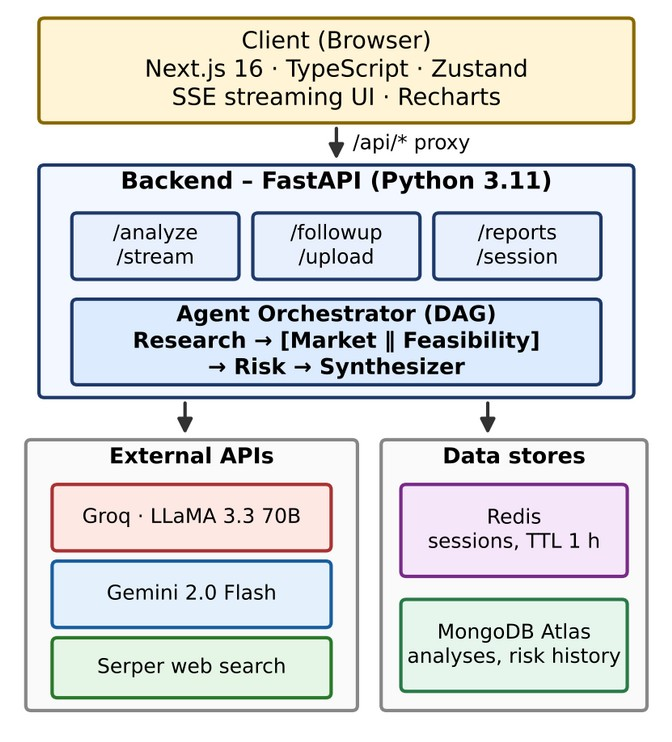
\includegraphics[width=0.92\columnwidth]{figs/vo_fig1.png}
\caption{VentureOS system architecture.}
\end{figure}

\begin{figure}[!t]
\centering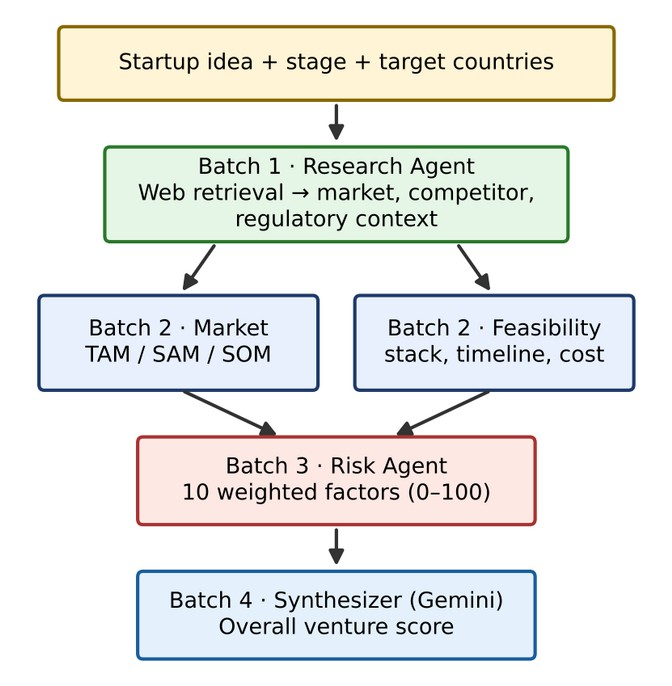
\includegraphics[width=0.85\columnwidth]{figs/vo_fig2.png}
\caption{Agent DAG with shared context.}
\end{figure}

\subsection{Agent Roster}
Five core agents always run; seven run on demand per dashboard tab (Table~II), exchanging schema-validated JSON.

\begin{table}[!t]
\caption{Agents and Their Outputs}
\centering\footnotesize
\begin{tabular}{@{}ll@{}}\toprule
\textbf{Agent} & \textbf{Output}\\\midrule
Research & Web evidence\\
Market Analysis & TAM/SAM/SOM, rivals\\
Feasibility & Stack, timeline, cost\\
Risk & Weighted score, band\\
Synthesizer & Venture score\\
Pitch Coach & Pitch score, strengths\\
Investment Planner & Stage, valuation\\
Team Recommender & Roles, hiring plan\\
Burn Rate & Burn, runway, budget\\
MVP / 90-Day & Features; weekly plan\\\bottomrule
\end{tabular}
\end{table}

\textit{Risk model.} The Risk Agent scores ten factors $s_i$ from 1 to 10, where 10 is lowest risk, each with a weight $w_i$ (Fig.~3): problem validity, market size and differentiation carry 10; regulatory, technical, team and financial runway carry 8; go-to-market, scalability and revenue model carry 6. With weights summing to 80,
\begin{equation}
R = 10\cdot\frac{\sum_i w_i s_i}{\sum_i w_i}\qquad(0\text{--}100).
\end{equation}
Bands: 70--100 low risk, 40--69 medium, 0--39 high (Table~III).

\subsection{Geography-Aware Modelling, Guardrails and Streaming}
Market size is computed for the selected countries in three tiers: TAM (total revenue opportunity), SAM (the reachable part) and SOM (obtainable in year one), with growth rate, maturity and competitor profiles; the Burn Rate Agent adjusts burn to local salaries. Advice depends on founder stage: students are pointed to hackathons, grants and accelerators (\$10K--\$100K asks), pre-seed startups to angels and micro-VCs (\$50K--\$500K). A Follow-up Agent answers only within the stored session. Results stream over Server-Sent Events [16] as each agent finishes.

\section{Results and Discussion}
\subsection{Functional Results}
For a submitted idea, VentureOS produces a complete venture report: market sizing with named competitors, a feasibility score with stack and cost, a risk score with per-factor breakdown, a pitch score with an elevator pitch, a burn-rate model, an MVP plan and a 90-day roadmap in four phases: Foundation (weeks 1--3), Build (4--7), Validate (8--10) and Launch (11--13). Because the pipeline streams, early agent results appear while later batches still run. Risk scores are stored in MongoDB, enabling per-idea history and cross-idea benchmarks through dedicated endpoints.

\subsection{Risk Weighting and Geographic Calibration}
Fig.~3 shows the risk weights; weighting problem validity, market size and differentiation highest reflects the view that building the wrong product dominates other failure causes [1]. Calibration changes financial conclusions materially: a \$50K budget lasts far longer when staffing in India than in the USA, so runway, SOM and team size differ for the same idea, and a global-average model would misstate cost for both. Table~III gives the cost ranges and score bands.

\begin{figure}[!t]
\centering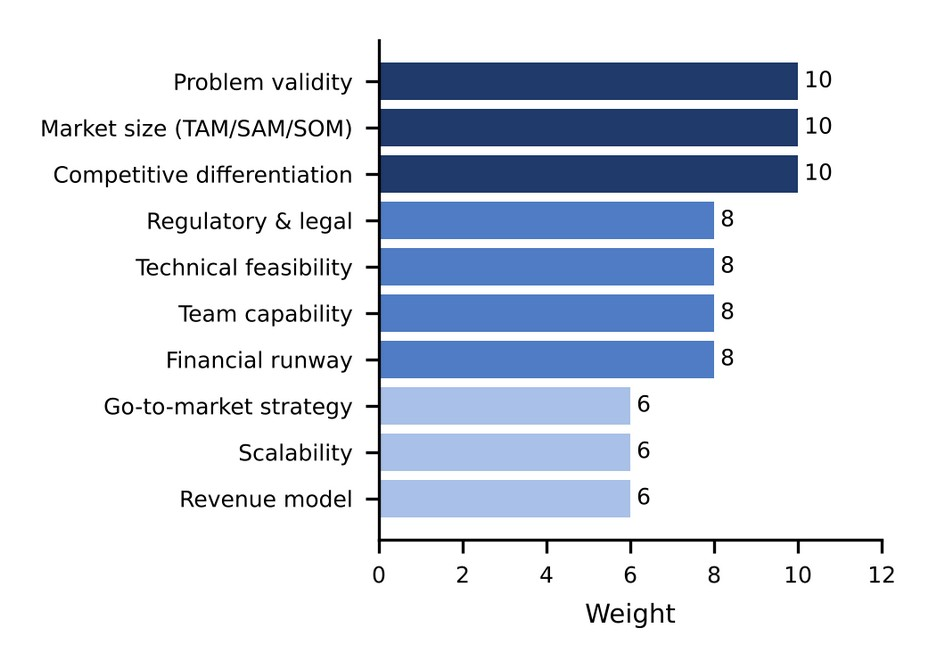
\includegraphics[width=0.9\columnwidth]{figs/vo_fig3.png}
\caption{Weights of the ten risk factors.}
\end{figure}

\begin{table}[!t]
\caption{Calibration Ranges and Score Bands}
\centering\footnotesize
\begin{tabular}{@{}ll@{}}\toprule
\textbf{Item} & \textbf{Value}\\\midrule
Engineer, India & \$800--\$2,500 / month\\
Engineer, USA & \$6,000--\$15,000 / month\\
Risk 70--100 & Low: fundable\\
Risk 40--69 & Medium: validate further\\
Risk 0--39 & High: pivot required\\\bottomrule
\end{tabular}
\end{table}

\subsection{Discussion}
\textit{Grounding.} Passing retrieved evidence downstream reduces dependence on parametric memory but does not eliminate error: search snippets can be outdated, biased towards well-indexed companies or wrong, and an LLM can still misread them. Competitor revenue and market-size figures are estimates to verify, not audited data.

\textit{Transparency of limits.} Weighted factor scores and bands show which assumption drives a recommendation, and stage-aware behaviour avoids one-size-fits-all advice. The weights, however, are design choices not yet calibrated against historical outcomes, and a high score does not predict success.

\textit{Robustness and cost.} Groq as fast primary model with Gemini as fallback improves availability, and parallel batches cut latency, but the system depends on three external APIs whose rate limits or outages affect results.

\subsection{Limitations and Threats to Validity}
No benchmark or user study is reported here. Factual accuracy of retrieved claims, agreement with expert analysts, end-to-end latency and user satisfaction remain to be measured. Outputs depend on LLM behaviour, which can change between model versions, and results for niche or non-English markets may be weaker because of sparser web evidence.

\section{Conclusion and Future Work}
\subsection{Conclusion}
VentureOS shows how a DAG of specialised, retrieval-grounded agents can turn a startup idea into a structured, stage-aware validation report in minutes. It exposes the limits of the analysis through weighted risk bands, geography-calibrated estimates and stage-specific guidance, and streams partial results so users can act on them early.

\subsection{Future Work}
Planned work includes: (1) evaluating factual accuracy and expert agreement on a labelled set of ideas; (2) calibrating risk weights against historical startup outcomes; (3) adding source citations and confidence indicators to every retrieved claim; (4) enabling abstention when retrieved evidence is insufficient; and (5) measuring latency, cost per analysis and user satisfaction in a user study.

\section*{References}
{\footnotesize\raggedright
\begin{enumerate}[label={[\arabic*]},leftmargin=2.2em,itemsep=1pt]
\item T. Eisenmann, ``Why start-ups fail,'' \textit{Harvard Business Review}, vol.~99, no.~3, pp.~76--85, 2021.
\item A. Vaswani et al., ``Attention is all you need,'' in \textit{Proc. NeurIPS}, 2017.
\item Z. Ji et al., ``Survey of hallucination in natural language generation,'' \textit{ACM Computing Surveys}, vol.~55, no.~12, pp.~1--38, 2023.
\item S. Kadavath et al., ``Language models (mostly) know what they know,'' arXiv:2207.05221, 2022.
\item P. Lewis et al., ``Retrieval-augmented generation for knowledge-intensive NLP tasks,'' in \textit{Proc. NeurIPS}, 2020.
\item Y. Gao et al., ``Retrieval-augmented generation for large language models: A survey,'' arXiv:2312.10997, 2023.
\item V. Karpukhin et al., ``Dense passage retrieval for open-domain question answering,'' in \textit{Proc. EMNLP}, 2020.
\item K. Shuster et al., ``Retrieval augmentation reduces hallucination in conversation,'' in \textit{Findings of EMNLP}, 2021.
\item S. Yao et al., ``ReAct: Synergizing reasoning and acting in language models,'' in \textit{Proc. ICLR}, 2023.
\item Q. Wu et al., ``AutoGen: Enabling next-gen LLM applications via multi-agent conversation,'' arXiv:2308.08155, 2023.
\item S. Hong et al., ``MetaGPT: Meta programming for a multi-agent collaborative framework,'' in \textit{Proc. ICLR}, 2024.
\item J. S. Park et al., ``Generative agents: Interactive simulacra of human behavior,'' in \textit{Proc. ACM UIST}, 2023.
\item A. Dubey et al., ``The Llama 3 herd of models,'' arXiv:2407.21783, 2024.
\item Gemini Team, Google, ``Gemini: A family of highly capable multimodal models,'' arXiv:2312.11805, 2023.
\item S. Ramirez, ``FastAPI documentation.'' [Online]. Available: \url{https://fastapi.tiangolo.com/}
\item WHATWG, ``HTML Living Standard: Server-sent events.'' [Online]. Available: \url{https://html.spec.whatwg.org/multipage/server-sent-events.html}
\end{enumerate}}
